\styledchapter[Architectuurontwerp van de oplossing]{architectuur-ontwerp-van-de-oplossing}
Nu het bekend is hoe ML pipelines en orkestratietools werken, kan er gekeken worden naar hoe de PoC architectonisch eruit gaat zien. De technische tekeningen laten zien hoe verschillende componenten in de PoC interacteren met elkaar en met componenten buiten de scope van de PoC. De tekeningen zijn gemaakt volgens het C4 model \cite{c4-model}. In dit hoofdstuk zal worden uitgelegd hoe C4 gelezen moet worden waarna de technische tekeningen wordt uitgelegd.

\section{Het C4 model}\label{sec:ch6-het-c4-model}
Het C4 model is een notatietechniek om de architectuur van een systeem te communiceren aan andere developers en is bedacht door Simon Brown \cite{c4-model}. Bij het tekenen van de modellen wordt er gedacht in vier niveaus: context, containers, components en code. In \autoref{fig:ch6-c4-overview-example} is een voorbeeld van een C4 model te zien. De context level is het eerste niveau waarbij wordt gekeken naar het systeem, gebruikers en contexten buiten de scope. Het systeem binnen de scope kan uitgebreid worden door middel van het volgende niveau: containers. Containers laten op een hoog niveau zien waar het systeem uit bestaat. Elk container kan verder verduidelijkt worden met het componentniveau. Hierbij worden containers verder opgebroken in components. Het laatste niveau is het code niveau en wordt doorgaans weergegeven via een klassendiagram. 

\begin{figure}[hbt!]
  \centering
  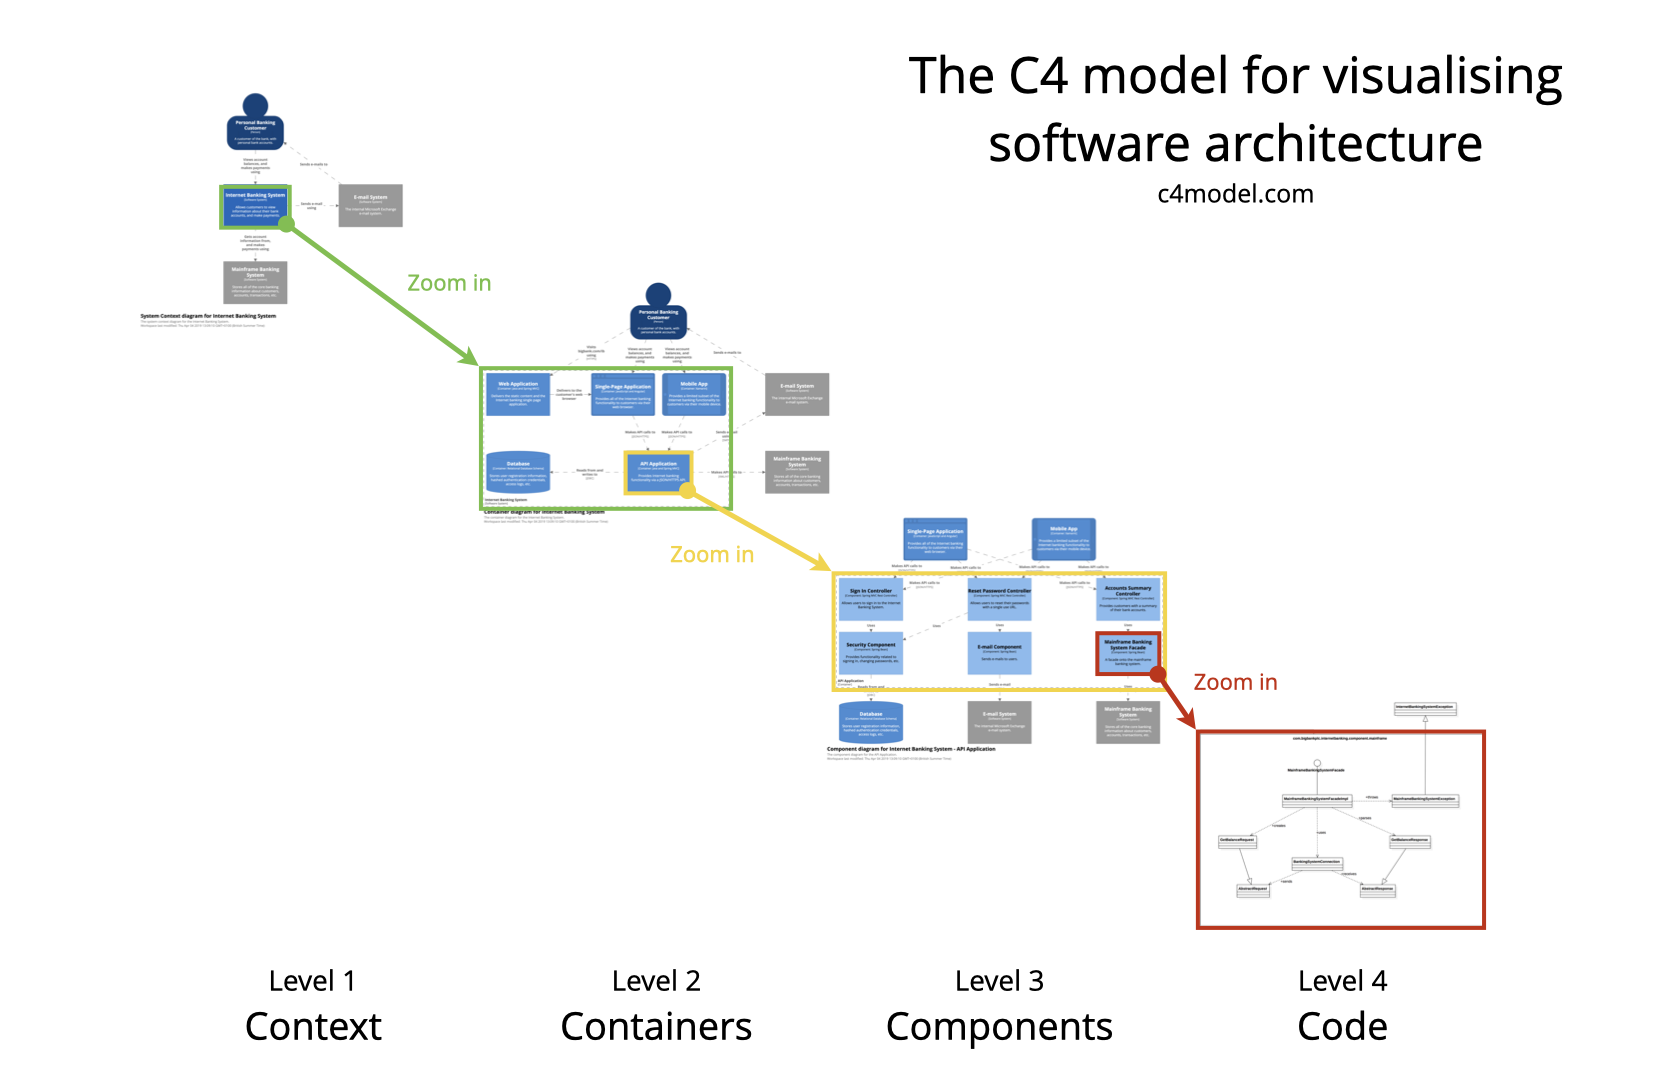
\includegraphics[width=0.99\textwidth]{chapter-6/c4-overview-example.png}
  \caption{Voorbeeld van een C4 model \cite{c4-model}}
  \label{fig:ch6-c4-overview-example}
\end{figure}

\newpage

\section{Architectuurontwerp}\label{sec:ch6-architectuurontwerp}
Op contextniveau is te zien dat het systeem, \acrfull{mlpa}, binnen de scope valt (\autoref{fig:ch6-c4-l1}). De scope is aangegeven met een stippellijn. Buiten de scope vallen de cloud platformen; het systeem interacteert met ze. In dit diagram is ook te zien dat developers alleen gebruik maken van het systeem en indirect van cloud platformen. In de context diagram is ook een \acrfull{cli}/program te zien dat gebruik kan maken van het \acrshort{mlpa} systeem. Deze valt echter buiten de scope en is daarom aangegeven met een stippellijn.

\begin{figure}[hbt!]
  \centering
  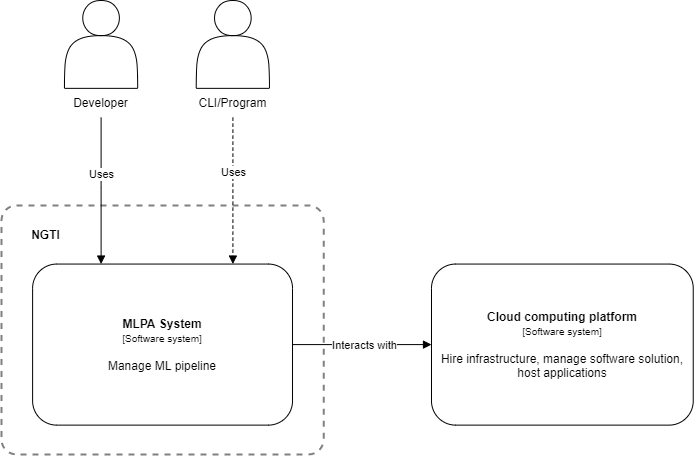
\includegraphics[width=0.65\textwidth]{chapter-6/C4-L1 - System Context diagram.png}
  \caption{Context niveau diagram van het architectuurontwerp}
  \label{fig:ch6-c4-l1}
\end{figure}

In \autoref{fig:ch6-c4-l2} is het container niveau van het \Acrshort{mlpa} systeem te zien. Het systeem bestaat uit een \acrfull{spa} front-end, een Node.js met Express back-end en een PostgreSQL database. Een developer krijgt van de back-end de \Acrshort{spa} geserveerd waarmee een pipeline beheert kan worden. De front-end stuurt \Acrshort{api} requests naar de back-end die vervolgens interacteert met de database en cloud platformen. Een \acrfull{erd} van het database is te vinden in \ref{appendix:erd}.

\newpage

\begin{figure}[hbt!]
  \centering
  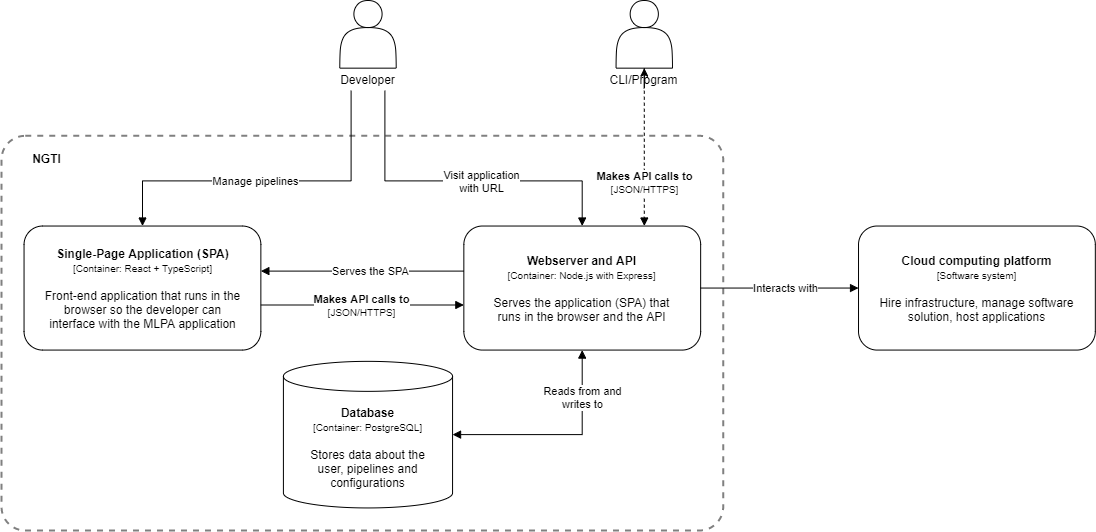
\includegraphics[width=0.99\textwidth]{chapter-6/C4-L2 - Container diagram.png}
  \caption{Container niveau diagram van het architectuurontwerp}
  \label{fig:ch6-c4-l2}
\end{figure}

Voor de keuze van frameworks is rekening gehouden met de populariteit en de  kwaliteit van documentatie. In \autoref{table:ch6-criteria-frameworks} zijn de criteria verder toegelicht.

\begin{table}[hbt!]
  \centering
  \caption{Criteria voor frameworks}
  \vspace*{.5\baselineskip}
  \begin{tabular}{|p{.15\linewidth}|p{.85\linewidth}|}
  \hline
  \textbf{Criteria} & \textbf{Toelichting} \\ \hline
    Populariteit
    &
    De populariteit zegt veel over hoe robuust een framework is. Hierbij wordt gekeken naar hoe vaak het framework wordt gebruikt en wie er achter het framework zit.
    \\ \hline

    Documentatie
    &
    De documentatie moet toegankelijk en duidelijk zijn. Ook moet de documentatie moet tutorials, concepten en een reference bevatten.
    \\ \hline
  \end{tabular}
  \label{table:ch6-criteria-frameworks}
\end{table}

Voor de opties is nogmaals de enquête van Stack Overflow geraadpleegd \cite{stack-overflow-survey-2020}. React, Angular en Vue zijn de meest gebruikte frameworks \cite{stack-overflow-survey-2020-technology-web-frameworks}. Angular is het minst gewild uit de drie opties \cite{stack-overflow-survey-2020-technology-most-loved-dreaded-and-wanted-languages} en is daardoor niet meegenomen in de keuze. Voor de backend zijn er twee opties: Node.js en .NET Core \cite{stack-overflow-survey-2020-popular-framework-libraries-tools}. In \autoref{table:ch6-criteria-compared-against-frontend-frameworks} zijn de front-end frameworks tegen de criteria gehouden en in \autoref{table:ch6-criteria-compared-against-backend-frameworks} de back-end frameworks.

\newpage

\begin{table}[hbt!]
  \centering
  \caption{Criteria tegen front-end frameworks}
  \vspace*{.5\baselineskip}
  \begin{tabular}{|p{.15\linewidth}|p{.4\linewidth}|p{.4\linewidth}|}
  \hline
  \textbf{Framework} & \textbf{Populariteit} & \textbf{Documentatie} \\ \hline
    \textbf{React} &
    Gebruikt door 35.9\% van developers volgens enquête \cite{stack-overflow-survey-2020-technology-web-frameworks}. Framework \newline gemaakt door Facebook. &
    Zeer uitgebreide documentatie met \newline tutorials, references en migration guides \cite{reactjs-docs}
    \\ \hline
    
    \textbf{Vue} &
    Gebruikt door 17.3\% van developers volgens enquête \cite{stack-overflow-survey-2020-technology-web-frameworks}. Framework \newline gemaakt door Evan You. & 
    Zeer uitgebreide documentatie met \newline tutorials, references en migration guides \cite{vue-docs}
    \\ \hline
  \end{tabular}
  \label{table:ch6-criteria-compared-against-frontend-frameworks}
\end{table}

\begin{table}[hbt!]
  \centering
  \caption{Criteria tegen back-end frameworks}
  \vspace*{.5\baselineskip}
  \begin{tabular}{|p{.15\linewidth}|p{.4\linewidth}|p{.4\linewidth}|}
  \hline
  \textbf{Framework} & \textbf{Populariteit} & \textbf{Documentatie} \\ \hline
    \textbf{Node.js} &
    Gebruikt door 51.4\% van developers volgens enquête \cite{stack-overflow-survey-2020-popular-framework-libraries-tools}. Framework \newline gemaakt door OpenJS Foundation. &
    Beknopte documentatie met reference en tutorials \cite{nodejs-docs}.
    \\ \hline

    \textbf{.NET Core} &
    Gebruikt door 26.7\% van developers volgens enquête \cite{stack-overflow-survey-2020-popular-framework-libraries-tools}. Framework \newline gemaakt door Microsoft. &
    Uitgebreide maar overweldigende \newline documentatie \cite{dotnet-core-docs}.
    \\ \hline
  \end{tabular}
  \label{table:ch6-criteria-compared-against-backend-frameworks}
\end{table}

React en Vue hebben beide sterke documentatie. Echter wordt React vaker gebruikt dan Vue; voor de front-end is gekozen voor React. De keuze voor het framework van de back-end is makkelijker te maken. De documentatie van .NET Core is uitgebreid maar kan snel overweldigend omdat er zo veel is. Voor de back-end is gekozen voor Node.js.

De component overview van de \acrshort{spa} is te zien in \autoref{fig:ch6-c4-l3-spa} en van de webserver met \acrshort{api} in \autoref{fig:ch6-c4-l3-nodejs}. De \acrshort{spa} bevat een \(AuthManager\) component dat controleert of de developer is ingelogd. Als dat het geval is, stuurt de \(Router\) component de developer door naar de \textit{Dashboard}, \textit{Pipeline overview} of \textit{Pipeline details} pagina.

\newpage

\begin{figure}[hbt!]
  \centering
  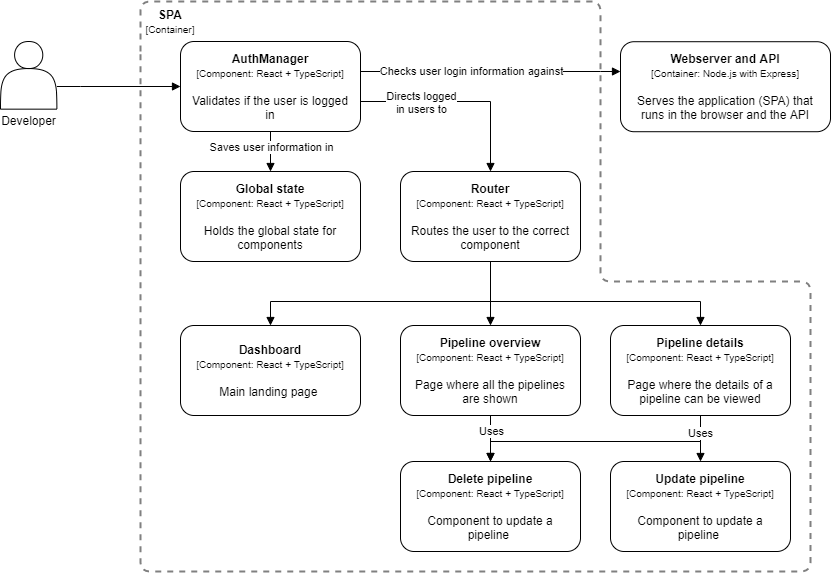
\includegraphics[width=0.8\textwidth]{chapter-6/C4-L3 - Component diagram - SPA.png}
  \caption{\Acrfull{spa} componentniveau diagram van het architecturaal ontwerp}
  \label{fig:ch6-c4-l3-spa}
\end{figure}

Het component diagram van de Node.js server bevat het complexe gedeelte (\autoref{fig:ch6-c4-l3-nodejs}). Hier komt een \acrshort{api} request binnen in een \(Express Route\). De route maakt vervolgens gebruik van Pulumi en de database om taken uit te voeren zoals het starten van een pipeline, het uploaden van een dataset of de status van een run bekijken.

\newpage

\begin{figure}[hbt!]
  \centering
  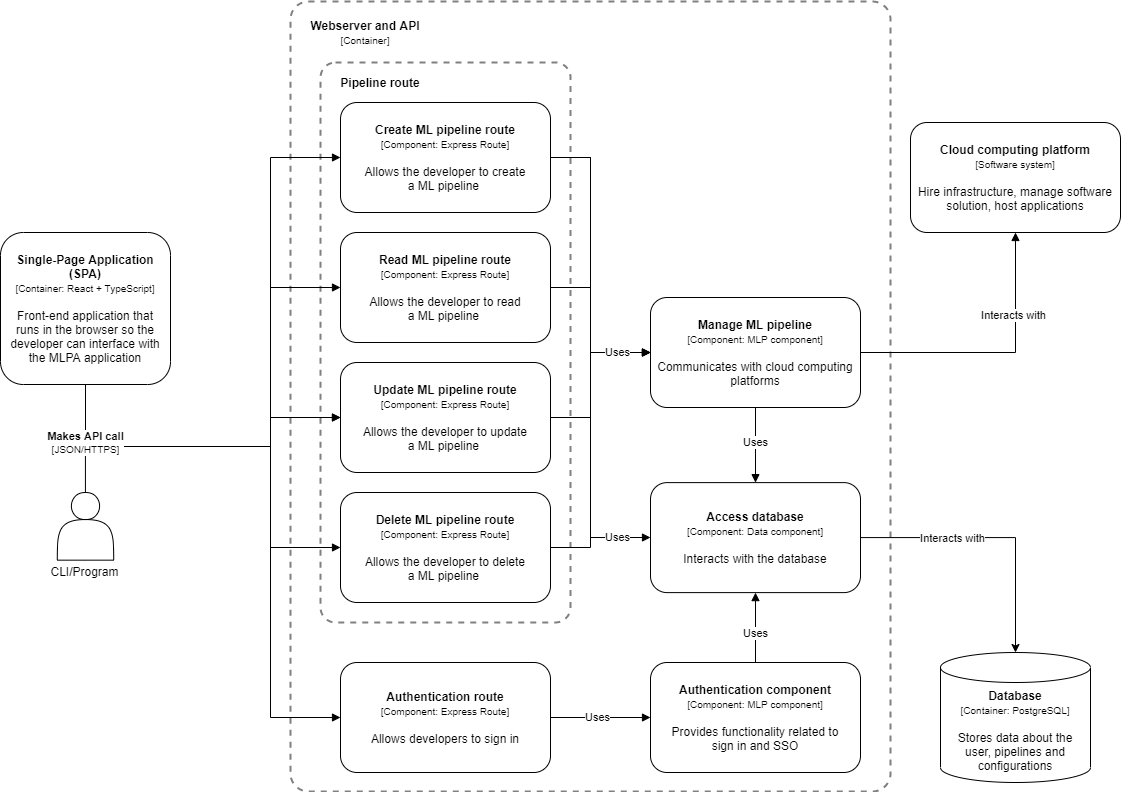
\includegraphics[width=0.99\textwidth]{chapter-6/C4-L3 - Component diagram - Webserver and API.png}
  \caption{Node.js server componentniveau diagram van het architecturaal ontwerp}
  \label{fig:ch6-c4-l3-nodejs}
\end{figure}

De architectuur van de Node.js server is ontworpen volgens het repository-service pattern \cite{repository-service-pattern}. Dit is een pattern dat bepaalde zaken van elkaar scheidt zodat het project onderhoudbaar blijft. In \autoref{sec:ch7-kwaliteit-van-de-code} zal dit uitgelegd worden met voorbeelden.

Diagrammen voor het laatste niveau, code, zijn achterwege gelaten omdat klassen niet worden gemaakt. In plaats daarvan worden functies gebruikt om een taak uit te voeren. Brown geeft ook als advies om de klassendiagrammen niet te maken of automatisch te laten genereren \cite{c4-model-faq} omdat de diagrammen vaak tijdens het programmeerproces zullen veranderen. Als alternatief voor de klassendiagrammen is gekozen om sequence diagrammen te maken om een beeld te geven wat er gebeurd op codeniveau.

\section{Sequence diagrammen}\label{sec:ch6-sequence-diagrammen}
Sequence diagrammen zijn gemaakt om het laatste niveau uit te leggen. Voor belangrijke acties zoals het aanmaken of uitvoeren van een pipeline is een sequence diagram gemaakt. Daarnaast is een \acrshort{erd} (bijlage \ref{appendix:erd}) gemaakt om de structuur van de database weer te geven. In deze paragraaf wordt er door een aantal diagrammen gelopen.

In \autoref{fig:ch6-c4-sd-create-pipeline} is te zien wat er gebeurt als een pipeline wordt aangemaakt. De developer stuurt een request naar de back-end waar het wordt gevalideerd. De validatie sequence diagram is te vinden in bijlage \ref{appendix:validation-sequence-diagram}. De back-end slaat vervolgens de gegevens op waarna, in parallel, een ingest server, model server en storage bucket worden aangemaakt. De ingest server zorgt voor de intake van datasets, de model server traint het model en in de storage bucket worden alle datasets en modellen opgeslagen. Als deze drie resources zijn aangemaakt, wordt de request voltooid.

\begin{figure}[hbt!]
  \centering
  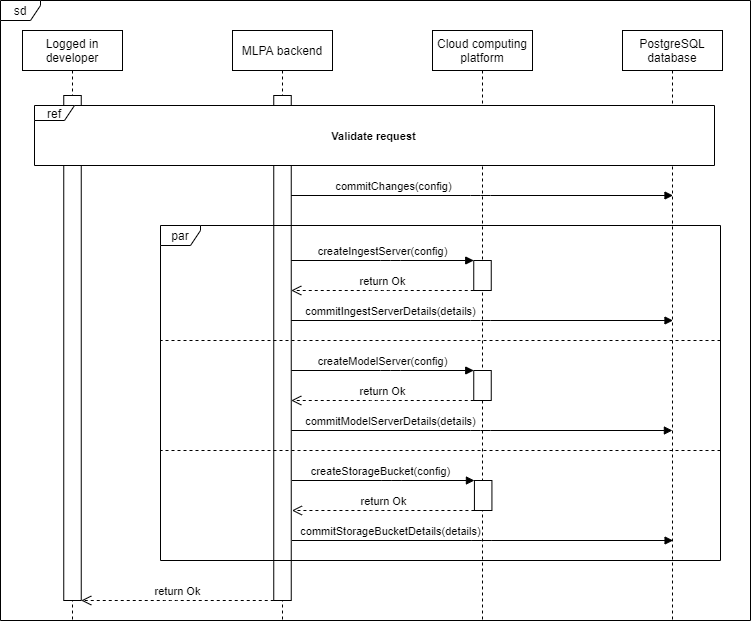
\includegraphics[width=0.99\textwidth]{chapter-6/C4-SD - Create pipeline.png}
  \caption{Sequence diagram van het aanmaken van een pipeline}
  \label{fig:ch6-c4-sd-create-pipeline}
\end{figure}

Een sequence diagram is gemaakt om te laten zien wat er gebeurt als een pipeline wordt gestart (\autoref{fig:ch6-c4-sd-start-pipeline}). De developer zal een request maken om de pipeline te starten. Om dit te doen stuurt de back-end een request naar de cloud platform om een \acrfull{vm} te starten. Na het opstarten wordt het trainen van het model automatisch gestart. De back-end past de status van de pipeline aan en voltooit de request. De developer weet nu dat een \acrshort{vm} is gestart en kan vragen naar de output van de \acrshort{vm}. In de output is te zien waar de \acrshort{vm} mee bezig is. Dit gebeurt continu totdat het model getraind is en de artefacten veilig zijn opgeslagen. Dit zijn afbeeldingen, modellen en datasets die bewaard moeten worden. Hierna zal de developer een laatste request sturen om de \acrshort{vm} te verwijderen en de status in de database aan te passen.

\clearpage

\begin{figure}[hbt!]
  \centering
  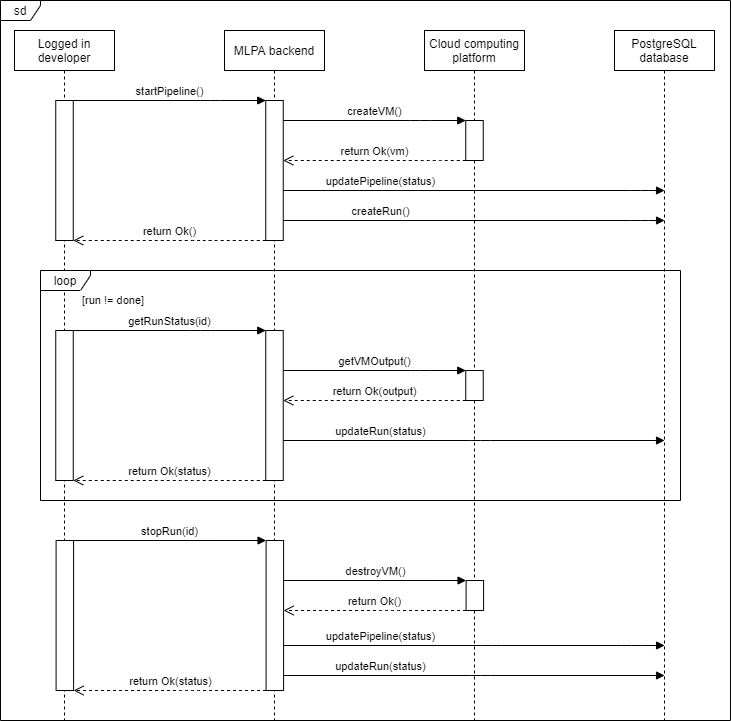
\includegraphics[width=0.99\textwidth]{chapter-6/C4-SD - Start pipeline.png}
  \caption{Sequence diagram van het starten van een pipeline}
  \label{fig:ch6-c4-sd-start-pipeline}
\end{figure}

